% !TEX root = master_thesis.tex
\chapter{Experimental Setup}
Here comes the very good text.
\section{Overview of the CBELSA/TAPS experiment}
\begin{figure}[htbp]
	\centering
	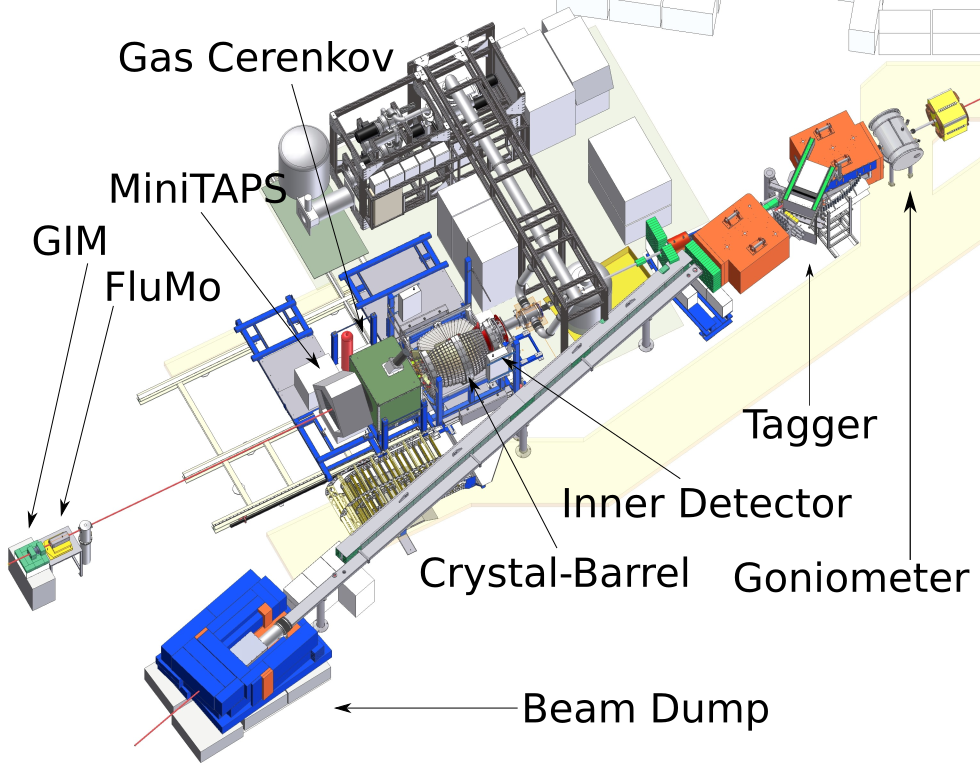
\includegraphics[width=\linewidth]{figs/CB-Area.png}
	\caption{Overview of the CBELSA/TAPS experiment \cite{cb}}
\end{figure}
\section{Production of (polarized) high energy photon beam}
\begin{figure}[htbp]
	\centering
	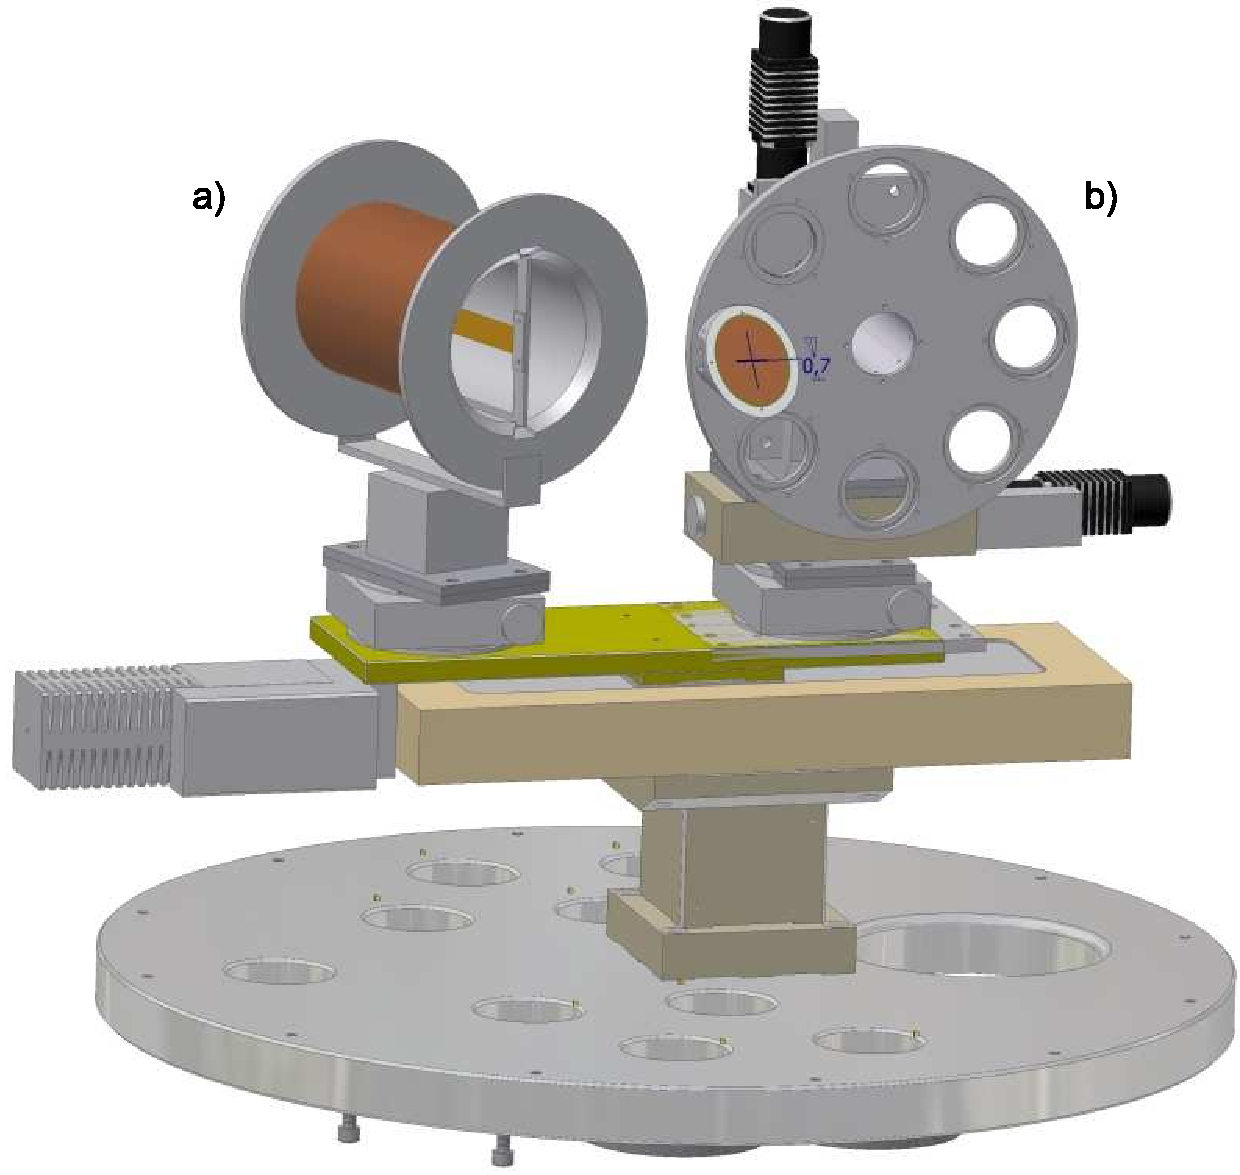
\includegraphics[width=.49\linewidth]{figs/goni-ganz.pdf}
	\caption{\cite{cb}}
\end{figure}
\begin{figure}[htbp]
	\centering
	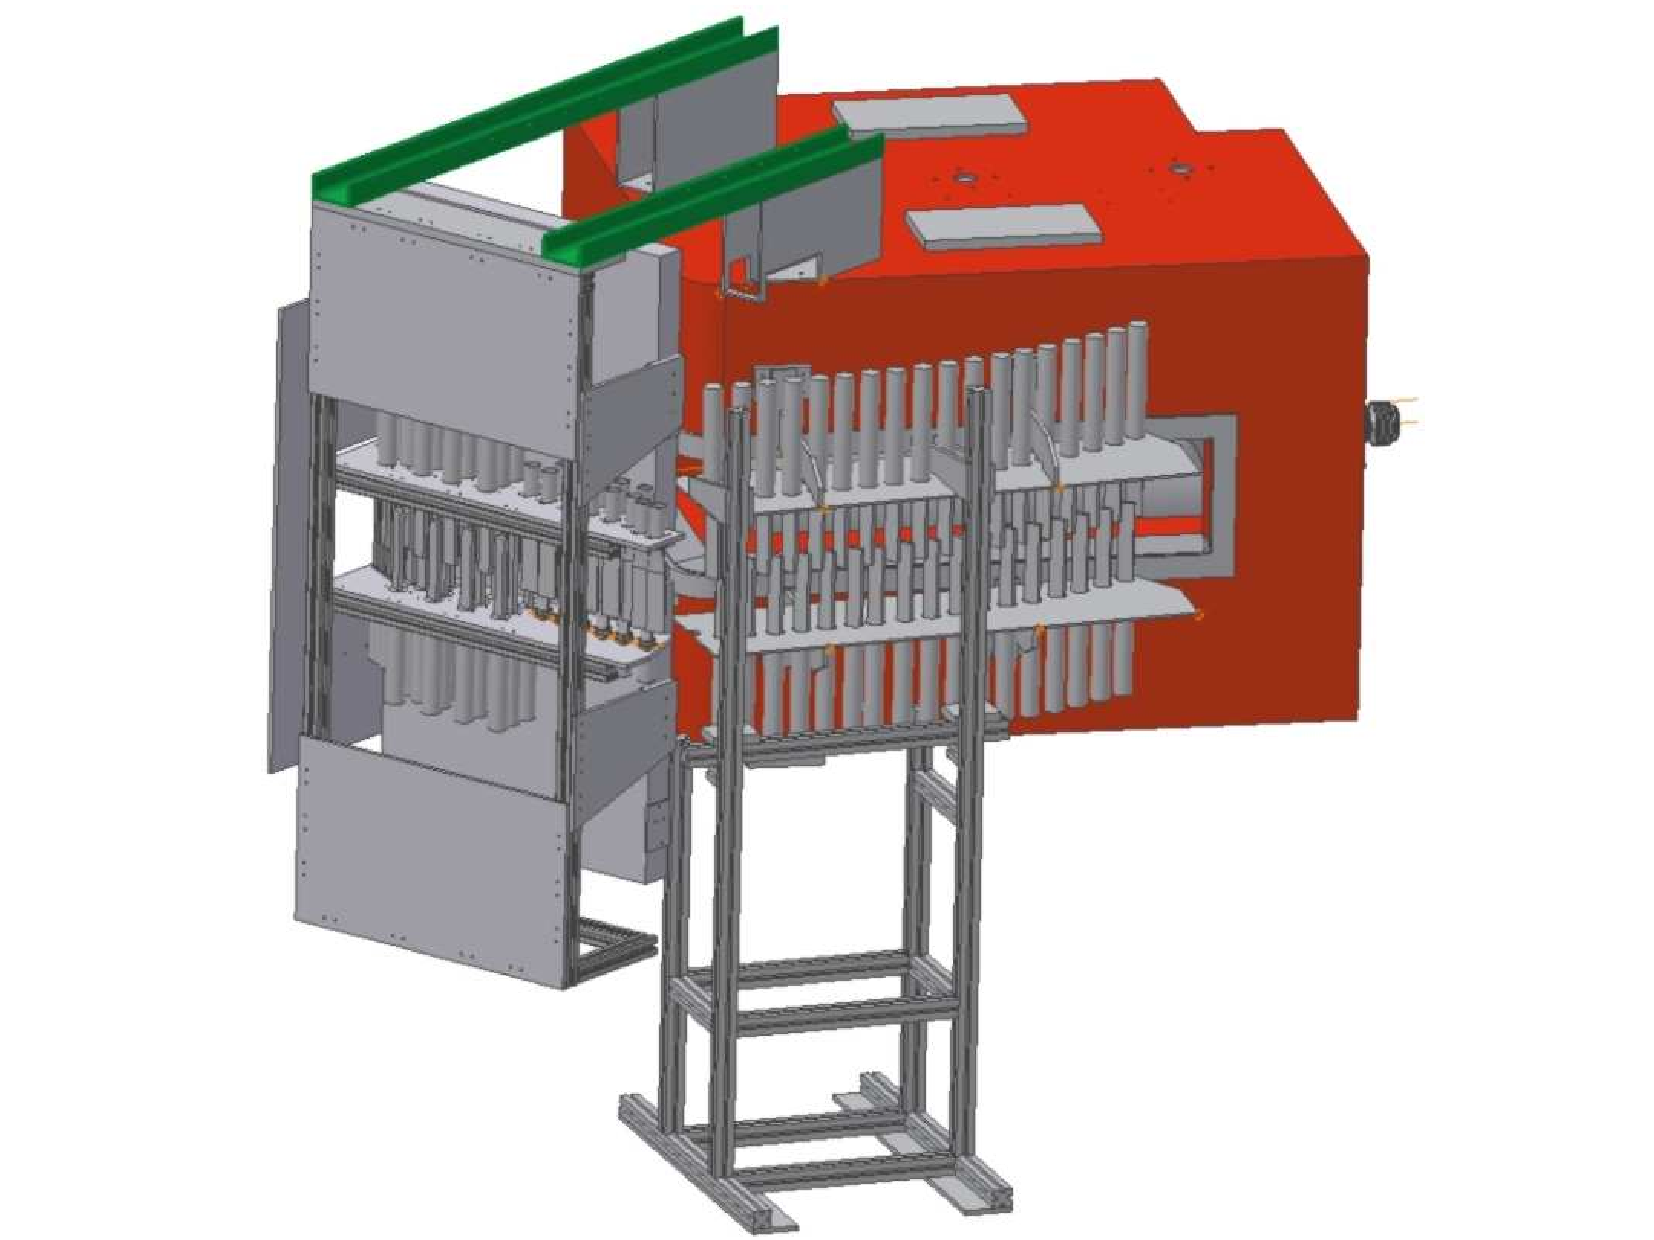
\includegraphics[width=.49\linewidth]{figs/Tagger.pdf}
	\caption{\cite{cb}}
\end{figure}

\section{Beam Target}

\begin{figure}[htbp]
	\centering
	\includegraphics[width=.5\linewidth]{figs/Target.pdf}
	\caption{\cite{cb}}
\end{figure}
\section{Calorimeters}
\begin{figure}[htbp]
	\centering
	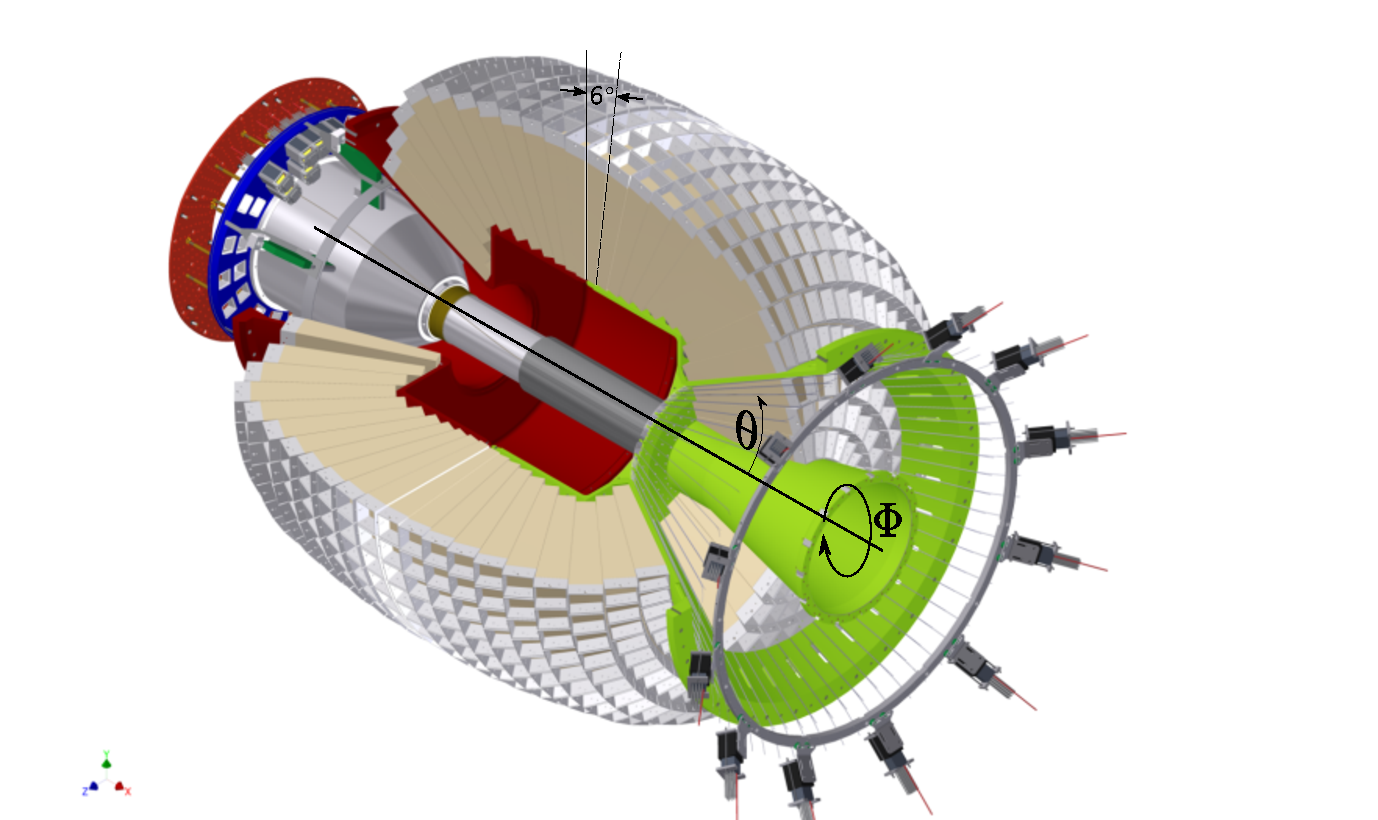
\includegraphics[width=\linewidth]{figs/cb_fp_in.pdf}
	\caption{\textsc{D. Walther} in \cite{urban}}
\end{figure}
\begin{figure}[htbp]
	\centering
	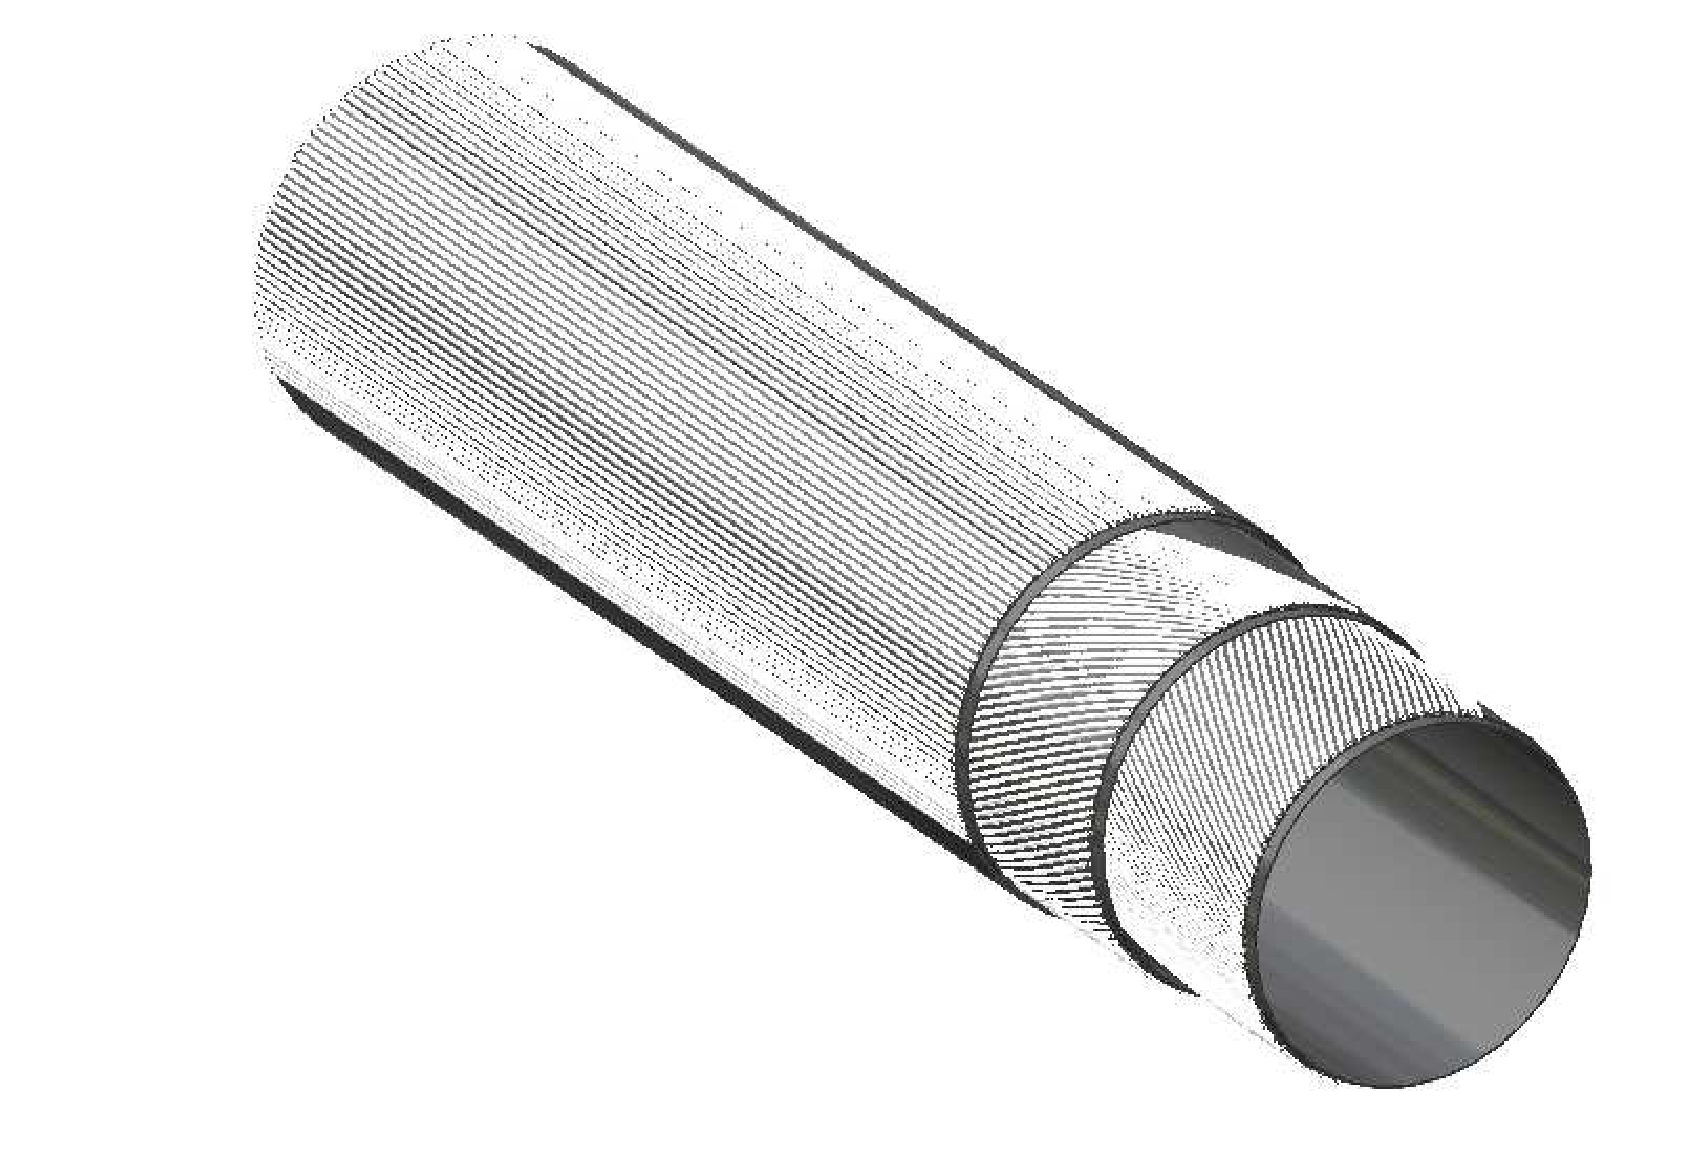
\includegraphics[width=.5\linewidth]{figs/faserorient.pdf}
	\caption{\cite{cb}}
\end{figure}
\begin{figure}[htbp]
	\centering
	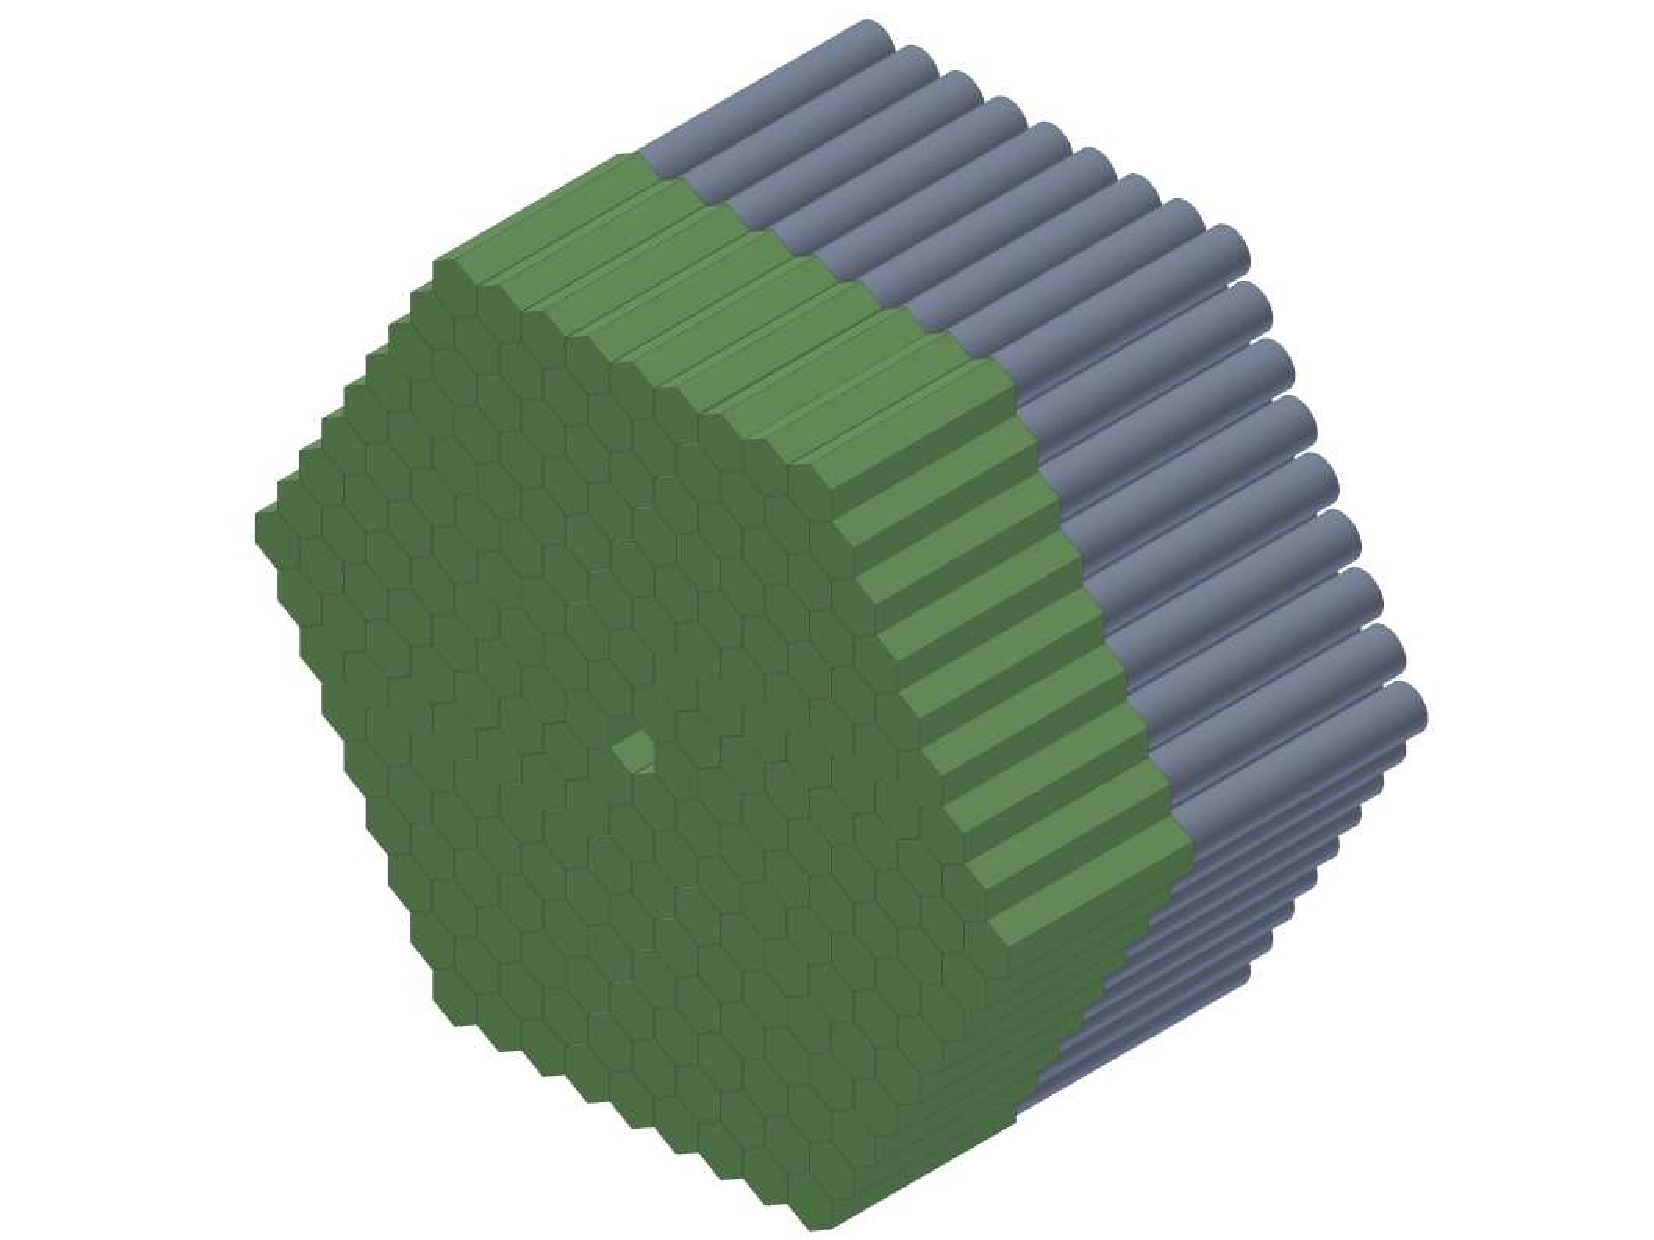
\includegraphics[width=.5\linewidth]{figs/mini-taps.pdf}
	\caption{\cite{cb}}
\end{figure}

\section{Trigger}